\documentclass[prl,onecolumn,floatfix,10pt,superscriptaddress]{revtex4-2}
%{quantumarticle}
%\pdfoutput=1
\usepackage[english]{babel}
\usepackage{amsmath}
\usepackage{bbm}
\usepackage{verbatim}
\usepackage{graphicx} 
\usepackage{amssymb}
\usepackage[colorlinks=true,citecolor=blue,linkcolor=blue,urlcolor=blue,pdfencoding=auto]{hyperref}
\usepackage[sort&compress]{natbib}
%\usepackage[numbers,sort&compress]{natbib}
\usepackage{xcolor}
\usepackage{orcidlink}

%\newcommand{\code}[1]{\texttt{#1}}
\newcommand{\code}[1]{\text{\texttt{#1}}}

% For comments
\definecolor{mcrcolor}{rgb}{0.7,0.2,0.7}
\definecolor{aprcolor}{rgb}{0.7,0.1,0.2}
\definecolor{philcolor}{rgb}{0.2,0.6,0.2}
\newcommand{\aprc}[1]{{\color{aprcolor}{[APR: #1]}}}
\newcommand{\pgc}[1]{{\color{philcolor}{[P: #1]}}}
\newcommand{\dptc}[1]{{\color{RoyalBlue}{[D: #1]}}}
\newcommand{\mcrc}[1]{{\color{mcrcolor}{[MCR: #1]}}}
\newcommand{\aglc}[1]{{\color{red}{[AGL: #1]}}}

\newcommand{\ket}[1]{\ensuremath{\left|{#1}\right\rangle}}
\newcommand{\bra}[1]{\ensuremath{\left\langle{#1}\right|}}
\newcommand{\msf}[1]{\mathsf{#1}}
\newcommand{\mcl}[1]{\mathcal{#1}}
\newcommand{\bsb}[1]{\boldsymbol{#1}}
\newcommand{\mbf}[1]{\mathbf{#1}}
%\newcommand{\mathbbm}[1]{\text{\usefont{U}{bbm}{m}{n}#1}}
\newcommand{\mymathbb}[1]{\text{\usefont{U}{bbold}{m}{n}#1}}

%\DeclareSymbolFont{greekletters}{OML}{FiraSans}{m}{n} 	

\newcommand{\bomega}{{\bar{\omega}}}

\newcommand{\mcH}{{\mcl{H}}}
\newcommand{\mcL}{{\mcl{L}}}
\newcommand{\mcG}{{\mcl{G}}}

\newcommand{\mcQ}{{\mcl{Q}}}
\newcommand{\mcW}{{\mcl{W}}}
\newcommand{\mcP}{{\mcl{P}}}
\newcommand{\mcR}{{\mcl{R}}}

\newcommand{\msF}{{\msf{F}}}
\newcommand{\msH}{{\msf{H}}}
\newcommand{\msG}{{\msf{G}}}
\newcommand{\msQ}{{\msf{Q}}}
\newcommand{\msP}{{\msf{P}}}

\newcommand{\msk}{{\msf{k}}}

\newcommand{\bu}{{\bsb{u}}}
\newcommand{\bv}{{\bsb{v}}}

\newcommand{\ba}{{\bsb{a}}}
\newcommand{\bh}{{\bsb{h}}}

\newcommand{\bxi}{{\bsb{\xi}}}

\newcommand{\rmout}{{{\rm out}}}
\newcommand{\rmin}{{{\rm in}}}

\newcommand{\mone}{{\mathbbm{1}}}




\begin{document}

\title{Floquet Topological Frequency-Converting Amplifier}

\author{Adrian Parra-Rodriguez\,\orcidlink{0000-0002-0896-9452}}
\email{adrian.parra.rodriguez@gmail.com}
\affiliation{Instituto de F\'isica Fundamental (IFF), CSIC, Calle Serrano 113b, 28006 Madrid, Spain.}
\affiliation{Technical University of Munich, TUM School of Natural Sciences, Physics Department, 85748 Garching, Germany}
\affiliation{Walther-Meißner-Institut, Bayerische Akademie der Wissenschaften, 85748 Garching, Germany}
\affiliation{Munich Center for Quantum Science and Technology (MCQST), 80799 Munich, Germany}
\author{Miguel Clavero-Rubio\,\orcidlink{0009-0002-7132-7097}}
\affiliation{Instituto de F\'isica Fundamental (IFF), CSIC, Calle Serrano 113b, 28006 Madrid, Spain.}
\author{Philippe Gigon\,\orcidlink{0009-0008-9802-9261}}
\affiliation{Technical University of Munich, TUM School of Natural Sciences, Physics Department, 85748 Garching, Germany}
\affiliation{Walther-Meißner-Institut, Bayerische Akademie der Wissenschaften, 85748 Garching, Germany}
\affiliation{Munich Center for Quantum Science and Technology (MCQST), 80799 Munich, Germany}
\author{Tom\'as Ramos\,\orcidlink{0000-0003-2182-7878}}
\affiliation{Instituto de F\'isica Fundamental (IFF), CSIC, Calle Serrano 113b, 28006 Madrid, Spain.}
\author{Álvaro Gómez-León\,\orcidlink{0000-0002-3990-5259}}
\affiliation{Instituto de F\'isica Fundamental (IFF), CSIC, Calle Serrano 113b, 28006 Madrid, Spain.}
\author{Diego Porras\,\orcidlink{0000-0003-2995-0299}}
\email{diego.porras@csic.es}
\affiliation{Instituto de F\'isica Fundamental (IFF), CSIC, Calle Serrano 113b, 28006 Madrid, Spain.}

\setcounter{equation}{0}
\setcounter{figure}{0}
\setcounter{table}{0}
\setcounter{page}{1}
\makeatletter
\renewcommand{\theequation}{S\arabic{equation}}
\renewcommand{\thefigure}{S\arabic{figure}}
\renewcommand{\bibnumfmt}[1]{[S#1]}
\renewcommand{\citenumfont}[1]{S#1}


\begin{center}
	{\large\bf Supplemental Material for ``Floquet Topological Frequency-Converting Amplifier''}
	
	\vspace{0.5cm}

	{
Adrian Parra-Rodriguez$^{1,2,3,4}$, 
Miguel Clavero-Rubio$^{1}$, 
Philippe Gigon$^{2,3,4}$, 
Tom\'as Ramos$^{1}$, 
Álvaro Gómez-León$^{1}$, 
Diego Porras$^{1}$
}

\vspace{0.3cm}

{\it
$^{1}$Instituto de F\'isica Fundamental (IFF), CSIC, Calle Serrano 113b, 28006 Madrid, Spain
$^{2}$Technical University of Munich, TUM School of Natural Sciences, Physics Department, 85748 Garching, Germany\\
$^{3}$Walther-Mei{\ss}ner-Institut, Bayerische Akademie der Wissenschaften, 85748 Garching, Germany\\
$^{4}$Munich Center for Quantum Science and Technology (MCQST), 80799 Munich, Germany
}

\end{center}

\section{Adiabatic elimination}
Here we derive the time-dependent quantum Langevin equation presented in Eq.~(2) of the main text, starting from a microscopic model in which the system mode $a$ is coupled to rapidly decaying auxiliary bosonic modes. A time-dependent coupling to one auxiliary mode generates an effective modulated decay channel for $a$, while a parametric coupling to a second fast-decaying mode yields an incoherent pump. Both constructions rely on standard adiabatic elimination in the Born-Markov regime.

\subsection{Time-dependent decay channel}

We first consider a single auxiliary mode $b$ that mediates time-dependent decay. The full system is governed by the Hamiltonian
\begin{align}
H = \omega_a a^\dagger a + \omega_b b^\dagger b +  g_b(t) (a^\dagger b + a b^\dagger),
\end{align}
where $g_b(t) = g_{b0} \cos(\Omega t/2)$ is a real-valued time-periodic coupling. The mode $b$ is coupled to a Markovian bath, resulting in fast decay at rate $\kappa_b$, and is taken to be initially in its vacuum state. We also allow mode $a$ to have its own intrinsic loss and (possibly) gain channels, as detailed in the main text.

We move to an interaction picture with respect to the free evolution of the uncoupled modes, defined by
\begin{align}
U_0(t) = \exp[-i(\omega_a a^\dagger a + \omega_b b^\dagger b)t].
\end{align}
In this frame, the interaction Hamiltonian becomes
\begin{align}
\tilde{H}_I(t) = -i g_b(t) \big(a^\dagger b e^{i \Delta_b t} - a b^\dagger e^{-i \Delta_b t}\big),
\end{align}
with $\Delta_b = \omega_b - \omega_a$ the detuning between the two modes. The Heisenberg equations of motion in this interaction picture are
\begin{align}
\dot{a}(t) &= -g_b(t) e^{i \Delta_b t} b(t), \\
\dot{b}(t) &=  g_b(t) e^{-i \Delta_b t} a(t) - \frac{\kappa_b}{2} b(t) +\sqrt{\kappa_b} b_{\text{in}}(t),
\end{align}
where $b_{\text{in}}(t)$ is the input noise operator driving the lossy auxiliary mode, with
$[b_{\text{in}}(t), b_{\text{in}}^\dagger(t')] = \delta(t - t')$.

We assume that the decay rate $\kappa_b$ is large compared to all other relevant energy scales
\begin{align}
\kappa_b \gg g_{b0},\, \Omega,\, \kappa_a,\, P,
\end{align}
so that $b$ can be adiabatically eliminated. Formally integrating the equation for $b(t)$ yields
\begin{align}
b(t) \approx \int_0^\infty d\tau\, e^{-\frac{\kappa_b}{2} \tau}
\left[ g_b(t - \tau) e^{-i \Delta_b (t - \tau)} a(t - \tau)
+ \sqrt{\kappa_b} b_{\text{in}}(t - \tau) \right].
\end{align}
Inserting this expression into the equation for $\dot{a}(t)$, and assuming that $g_b(t)$ and $a(t)$ vary slowly on the timescale $\kappa_b^{-1}$, we use the Markov approximation
$g_b(t - \tau) \approx g_b(t)$ and $a(t - \tau) \approx a(t)$ inside the integral. Evaluating the convolution yields
\begin{align}
\dot{a}(t)
= -\underbrace{\frac{g_b(t)^2}{\kappa_b/2 - i \Delta_b}}_{\Gamma_b(t)} a(t)
- g_b(t) e^{i \Delta_b t} \sqrt{\kappa_b} \int_0^\infty d\tau\, e^{-\frac{\kappa_b}{2} \tau} b_{\text{in}}(t - \tau).
\label{eq:adot_QLE_SM}
\end{align}
Writing $\Gamma_b(t) = \kappa(t)/2 + i\delta\omega(t)$, we identify the induced time-dependent decay rate and Lamb shift as
\begin{align}
\kappa(t) &= \frac{4 g_b(t)^2}{\kappa_b^2 + 4 \Delta_b^2}\kappa_b,\qquad
\delta\omega(t) = \frac{4 g_b(t)^2}{\kappa_b^2 + 4 \Delta_b^2}\Delta_b.
\end{align}
On resonance ($\Delta_b = 0$), this simplifies to
\begin{align}
\kappa(t) = \frac{4 g_b(t)^2}{\kappa_b}.
\end{align}
The second term in Eq.~\eqref{eq:adot_QLE_SM} represents an effective input-noise contribution, which can be written as a filtered noise operator. On resonance, it is well-approximated by
\begin{align}
\xi_{\text{aux}}(t)
= - g_b(t) \sqrt{\kappa_b} \int_0^\infty d\tau\, e^{-\frac{\kappa_b}{2} \tau} b_{\text{in}}(t - \tau)
\approx - \frac{2 g_b(t)}{\sqrt{\kappa_b}}\, b_{\text{in}}(t),
\end{align}
consistent with an effective decay channel of rate $\kappa(t)$.

\subsection{Incoherent pump channel}

An incoherent pump channel for $a$ can be engineered in a fully analogous way by coupling $a$ to a second fast-decaying auxiliary mode $c$ via a parametric (two-mode-squeezing) interaction~\cite{Roushan2017,Busnaina2024},
\begin{align}
H_P = \omega_c c^\dagger c + g_c (a^\dagger c^\dagger + a c),
\end{align}
with $c$ coupled to a Markovian bath at rate $\kappa_c$ and initialized in its vacuum state. Working in the appropriate rotating frame and applying the same adiabatic-elimination steps as above (now for $c$), one finds that for
\begin{align}
\kappa_c \gg g_c,\, \kappa_a,\, \kappa_b,\, \Omega,
\end{align}
the mode $c$ induces an effective incoherent pump for $a$ with rate
\begin{align}
P = \frac{4 g_c^2}{\kappa_c},
\end{align}
and an associated noise term $\sqrt{P}\, c_{\text{in}}^\dagger(t)$, where $c_{\text{in}}(t)$ denotes the corresponding input noise operator. This is the standard result for a negative-damping (gain) channel generated via a strongly damped parametric auxiliary mode.

\subsection{Full effective Langevin equation}

Including the intrinsic loss of mode $a$, the engineered time-dependent decay from mode $b$, and the incoherent pump from mode $c$, and restoring the possibly time-dependent system frequency $\omega_0(t)$, we obtain the effective Langevin equation
\begin{align}
\dot{a}(t)
= -i \omega_0(t) a(t)
+ \frac{P - (\gamma + \kappa(t))}{2}\, a(t)
+ \xi_\mathrm{in}(t),
\end{align}
with $\kappa(t) = \frac{4 g_b(t)^2}{\kappa_b}$, where $\gamma$ denotes any additional unmodulated loss channel. The total input noise operator is
\begin{align}
\xi_\mathrm{in}(t)
= -\sqrt{\kappa(t)}\, b_{\text{in}}(t)
  -\sqrt{\gamma}\, d_{\text{in}}(t)
  +\sqrt{P}\, c_{\text{in}}^\dagger(t),
\end{align}
with $d_{\text{in}}$ the input associated with the background loss channel. This Langevin equation coincides with Eq.~(2) in the main text and provides a microscopic justification for the effective model with time-dependent decay rate $\kappa(t)$ and incoherent pump $P$. The derivation is valid in the regime $\kappa_{b,c} \gg g_{b0}, g_c, \Omega, \kappa_a$ and under the usual Markov and adiabatic approximations, and it extends straightforwardly to more general slow modulations of $g_b(t)$ and $\omega_0(t)$. 

As an example, in Fig.~\ref{fig:time_dynamics}(a) we show a comparison between the transient of the real part of the averaged field amplitude $\alpha(t)=\langle a(t)\rangle$ computed by direct integration of the Langevin equation with a coherent input at port $\gamma$, $\langle d_\rmin(t)\rangle =  \alpha_d e^{-i\omega_d t}$ ($\omega_d = \bomega_d + n_d \Omega$) with $\alpha_d=\frac{\epsilon_d}{\sqrt{\gamma}}$, and all others in vacuum, with the reconstructed signal obtained from the Green's function formalism (Eq.~(3), i.e., 
\begin{align}
\langle \bar{a}_n(\bomega) \rangle &= \sqrt{2\pi} \epsilon_d\msf{G}_{n, n_d}(\bomega) \delta(\bomega - \bomega_d).
\label{eq:abar_wbar_Gnm}
\end{align}

In Fig.~\ref{fig:time_dynamics}(b), we show the time-integrated dynamics for the one-mode model and a more realistic three-mode model in cQED, with the two auxiliary modes in the very bad-cavity limit. Naturally, as we approach the topological singular regime ($\beta=1$) the auxiliary degrees of freedom become populated and the effective slow-dynamics deviates from the idealized case. 


\begin{figure}[h]
\centering
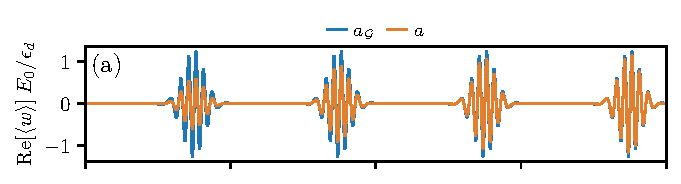
\includegraphics[width=.7\linewidth]{a_t_for_etaw=10.0_etak=20.0_etakp=10.0_etaP=19.8_f=1.0.pdf}
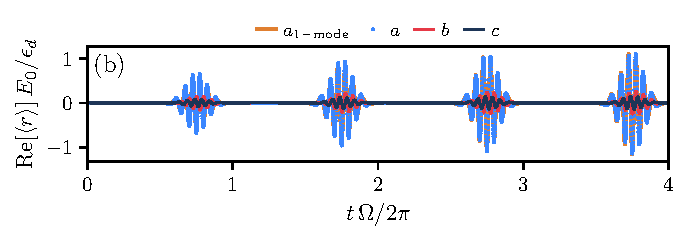
\includegraphics[width=.7\linewidth]{3mod_Simulation_etaw10_etak20_etagamma10_etaP19.8_phi0.5_kappa_b_200.0_kappa_c_1200.0.pdf}
\caption{(a) Transient dynamics 
for the real part of the averaged fields $\langle w(t)\rangle$, with 
$w\in\{a, a_{\mathcal G}\}$. The curve for the integrated Langevin equation~(2), $w=a$ (orange) approaches the 
steady-state response $w=a_{\mathcal G}$ 
(blue), obtained from the truncated Green’s function in 
Eq.~\eqref{eq:abar_wbar_Gnm}. Both quantities are normalized by the drive 
amplitude $\epsilon_d$ and by the singular value $|E_0| \approx 2.4\times10^{-3}$. 
Parameters are $\eta_\omega=\eta_\kappa=\eta_\gamma=10$, $\eta_P=19.8$ 
($\beta=0.98$), and $\phi=\pi/2$. As $\beta\to1$, the system requires 
increasingly long times to reach its steady state. (b) Time-domain comparison between the real part of the amplitudes in the three-mode model ($r=\{a,b,c\}$), and those of the effective (ideal) one-mode model ($r=\{a_{1-\mathrm{mode}}\}$). The parameters used for $a_{1-\mathrm{mode}}$ (and $a$) are the same as in panel (a). The $b$ and $c$ modes are resonant with $a$ and decay at rates $\kappa_b = 200\Omega$ and $\kappa_c = 1200\Omega$, with couplings $g_b(t)$ and $g_c$ chosen to reproduce $\eta_\kappa$ and $\eta_P$.}
\label{fig:time_dynamics}
\end{figure}



\section{Signal-to-noise ratio}
In this section, we first compute the signal-to-noise ratio if we measure the photon number. Using the input-output relation at the static port $\gamma$, the Floquet-Sambe components of the output field read
\begin{align}
\bar{d}_{\text{out},n}(\bar\omega) 
= \sum_m \Big[
\msf{R}_{n m}(\bar\omega)\, \bar{d}_{\text{in},m}(\bar\omega) + \msf{P}_{n m}(\bar\omega)\, \bar{h}_{\text{in},-m}^\dagger(-\bar\omega)
+ \msf{Q}_{n m}(\bar\omega)\, \bar{a}_{\text{in},m}(\bar\omega) 
\Big],
\end{align}
with coefficient matrices 
\begin{align}
\msf{R}_{n m}(\bar\omega) &= \delta_{n m} - i \Omega\,\eta_{\gamma}\,\msG_{n m}(\bar\omega),\qquad
% \msf{Q}_{n m}(\bar\omega)  &= -\,i\,\frac{\Omega\sqrt{\eta_\kappa\eta_{\gamma}}}{2}
% \big[\msf{G}_{n,m-1}(\bar\omega)+\msf{G}_{n,m+1}(\bar\omega)\big],\\
\msP_{n m}(\bar\omega) = i\,\Omega\sqrt{\eta_{P}\eta_{\gamma}}\,\msf{G}_{n m}(\bar\omega).
\end{align}
For simplicity, we assume that the $\kappa(t)$ port is in vacuum and omit the definition of $\msQ_{nm}(\bar{\omega})$; it follows straightforwardly from a Floquet--Fourier expansion with $\Omega/2$ spacing.


We now consider the case where the port $\gamma$ is driven with a monochromatic coherent tone $\ket{\alpha(\omega_d)}$ at $\omega_d=\bar\omega_d+n_d\,\Omega$, such that 
$\langle \bar d_{\rm in,m}(\bar\omega)\rangle = \sqrt{2\pi}\,\alpha_d\,\delta_{m,n_d}\,\delta(\bar\omega-\bar\omega_d),
$ while all other inputs remain in vacuum. The output photon flux can be split into a coherent contribution (\emph{signal}) and an incoherent one (\emph{noise}),
\begin{align}
\mcl{D}_{\rmout}(t)\equiv \langle d_{\rm out}{}^\dag(t)\,d_{\rm out}(t)\rangle
=\mcl{S}_{\rm out}(t)+\mcl{N}_{\rm out}(t),
\end{align}
with (cyclostationary) components
\begin{align}
\mcl{S}_{\rmout}(t)&=\left|\alpha_d\sum_n e^{-i n \Omega t} \msf{R}_{n,n_d}(\bar\omega_d)\right|^2,\\
\mcl{N}_{\rm out}(t)&=\frac{1}{2\pi} \sum_{n,m}e^{i(n-m)\Omega t}
\sum_{l}\int_0^{\Omega}\! d\bar\omega \;
\msf{P}^*_{n l}(\bar\omega)\,\msf{P}_{m l}(\bar\omega),
\end{align}
where only the incoherent-pump bath contributes to $\langle a^\dag a\rangle$, since the other input ports are at zero-temperature and enter exclusively through the matrix $\msf{P}_{nm}$.

\bibliographystyle{apsrev4-2}
\bibliography{main.bib}

\end{document}
